\documentclass{beamer}[10]

% ====================== Pacotes ====================== %
\usepackage{pgf}
\usepackage[utf8]{inputenc}
\usepackage[brazil]{babel}
\usepackage{beamerthemesplit}
\usepackage{graphics,epsfig, subfigure}
\usepackage{url}
\usepackage{srcltx}
\usepackage{hyperref}
% ====================== Pacotes ====================== %

% ======================= Tema ======================== %
\definecolor{kugreen}{RGB}{50,93,61}
\definecolor{kugreenlys}{RGB}{132,158,139}
\definecolor{kugreenlyslys}{RGB}{173,190,177}
\definecolor{kugreenlyslyslys}{RGB}{214,223,216}
\setbeamercovered{transparent}
\mode<presentation>
\usetheme[numbers,totalnumber,compress,sidebarshades]{PaloAlto}
\setbeamertemplate{footline}[frame number]

\usecolortheme[named=kugreen]{structure}
\useinnertheme{circles}
\usefonttheme[onlymath]{serif}
\setbeamercovered{transparent}
\setbeamertemplate{blocks}[rounded][shadow=true]
% ======================= Tema ======================== %

\title[Buzzmap]
{Buzzmap\\
Dependabilidade}
\author[dggc\\josue\\lfmendes]{Daniel Galinkin, Luiz Felipe Mendes, Victor Josué}

\institute[UFMG] % opcional
{Departamento de Ciência da Computação
\\Universidade Federal de Minas Gerais}

\subject{Dependabilidade}

\date{\today}

\begin{document}

   \frame{\titlepage}

   % Mostra um table of contents no inicio de cada subsection:
   \AtBeginSection[] {
     \begin{frame}<beamer>{Sumário}
       \tableofcontents[currentsection,currentsubsection]
     \end{frame}
   }
   \AtBeginSubsection[] {
     \begin{frame}<beamer>{Sumário}
       \tableofcontents[currentsection,currentsubsection]
     \end{frame}
   }

    
    \section{Introdução}    
    
    \frame[allowframebreaks]{
    
        \frametitle{O que é Buzzmap}
        \begin{itemize}
        \item Inteligência Competitiva em Redes Sociais 
        \item Medir o "Buzz" na Internet
        \item Análise de Marcas na Web
        \end{itemize}

        \framebreak

        \begin{block}{Exemplo}
            \begin{description}
                \item[Coca-Cola] A Coca-Cola deseja medir a repercussão da
                campanha "Prove que é possível!"
            \end{description}
        \end{block}
    }

    \frame{
    
        \frametitle{Como funciona}
        \begin{itemize}
        \item A ferramenta pesquisa e coleta todas as ocorrências relativas às
        ações da campanha, nas redes sociais como: YouTube, Flickr, Twitter
        \end{itemize}
    }

    
    \section{Descrição do sistema} 

    \subsection{Tipos de usuários}

    \frame{
        \frametitle{Tipos de usuários}
        \begin{itemize}
        \item Analista
        \item Cliente
        \end{itemize}
    }

    \subsection{Requisitos}

    \frame{
        \frametitle{Requisitos}
        \begin{itemize}
        \item A interface gráfica tem que ser acessível via um browser
            pela internet.
        \item Dado um conjunto de palavras chaves o sistema tem de ter a
            capacidade de coletar conteúdo em diversos canais(orkut, flickr,
            blog, twitter).
        \item O sistema deve ter uma interface gráfica que mostra o
            conteudo coletado.
        \item O sistema deve ter uma interface que dá capacidade de se
            analisar o conteúdo coletado.
        \item O sistema deve ser capaz de gerar gráficos sobre a análise
            feita.
        \end{itemize}
    }

    \subsection{Requisitos de Dependabilidade}

    \frame{
        \frametitle{Requisitos de Dependabilidade}

        \begin{description}
            \item[Disponibilidade do servidor] O sistema tem que ficar no ar
            durante pelo menos 90\% do tempo durante os horários de análise -
            8:00 as 20:00.
            \item[Safety] O sistema deve fazer um backup do banco de dados de
            12 em 12 horas.
            \item[Security] O sistema deve manter dados de usuários(login e
            senhas) protegidos.
            \item[Security] O sistema deve ter uma divisão de privilégios,
            sendo que algumas informações só podem ser vistas por certos
            usuários.
        \end{description}
    }

    \subsection{Atores}
    \frame{
        \frametitle{Atores}
        \begin{itemize}
        \item Desenvolvedor
        \item Administrador
        \item Analista
        \item Cliente
        \end{itemize}
    }

    \subsection{Casos de uso}
    \frame{
        \frametitle{Exemplo}
        \begin{figure}
            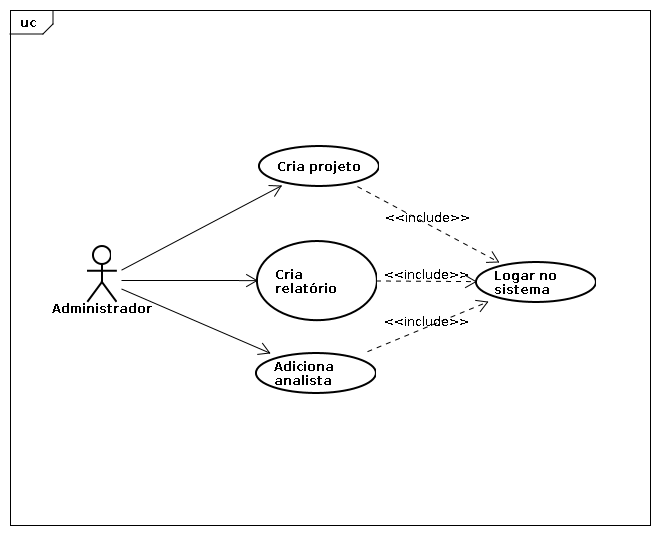
\includegraphics[width=0.7\textwidth]{img/caso-uso-administrador.png}
            \caption{Diagrama dos casos de uso do administrador do sistema}
            \label{fig:admin}
        \end{figure}

    }


    \subsection{Diagrama de atividades}
    \frame{
        \frametitle{Exemplo}
        \begin{figure}
            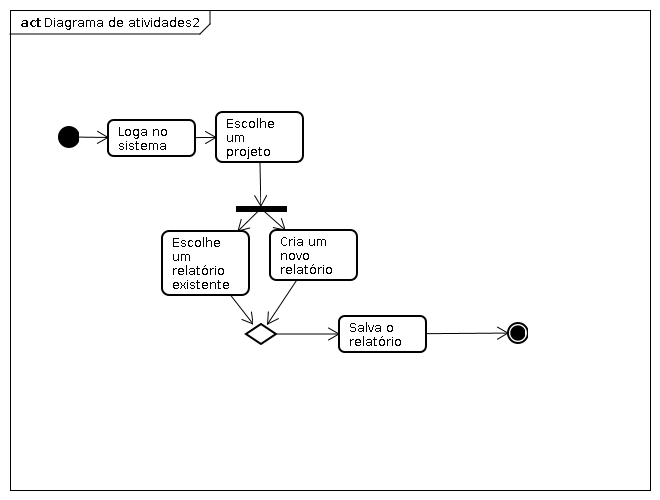
\includegraphics[width=0.7\textwidth]{img/atividade2.png}
            \caption{Diagrama de atividades de criação/seleção de
                relatórios}
            \label{fig:ativ}
        \end{figure}

    }

    \subsection{Visão de arquitetura e componentes}

    \frame[allowframebreaks]{
    
        \frametitle{Arquitetura}

        \begin{figure}
            \begin{center}
                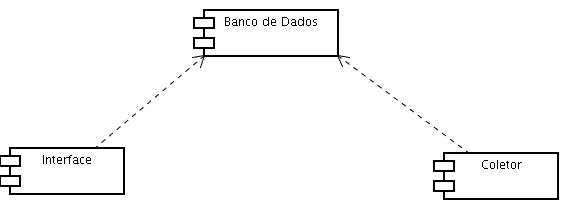
\includegraphics[width=0.7\textwidth]{img/conceitual}
                \caption{Arquitetura conceitual geral do sistema}
                \label{fig:arquitetura-conceitual}
            \end{center}
        \end{figure}

        \framebreak

        \begin{figure}
            \begin{center}
                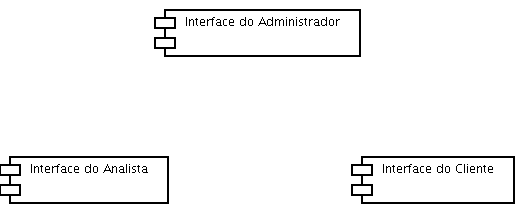
\includegraphics[width=0.7\textwidth]{img/interface}
                \caption{Arquitetura dos subsistemas da interface}
                \label{fig:arquitetura-interface}
            \end{center}
        \end{figure}

        \framebreak

        \begin{figure}
            \begin{center}
                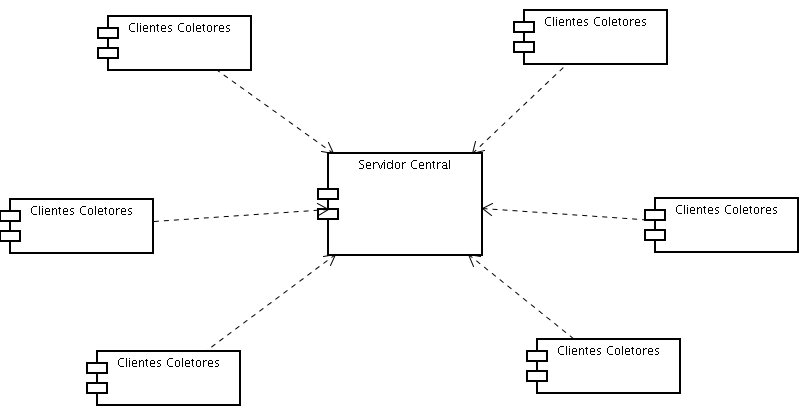
\includegraphics[width=0.7\textwidth]{img/coletor}
                \caption{Arquitetura dos subsistemas do coletor}
                \label{fig:arquitetura-coletor}
            \end{center}
        \end{figure}

        \framebreak

        \begin{figure}
            \begin{center}
                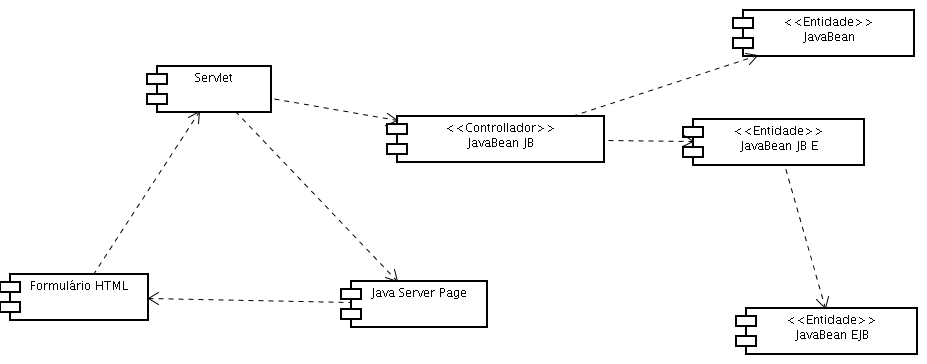
\includegraphics[width=0.7\textwidth]{img/jsp}
                \caption{Visão de camadas da implantação JSP}
                \label{fig:arquitetura-jsp}
            \end{center}
        \end{figure}
    }


    \section{Prism}

    \subsection{Máquina de estados}
    \frame[allowframebreaks]{
    
        \frametitle{Máquina de estados}
        \begin{figure}
            \begin{center}
                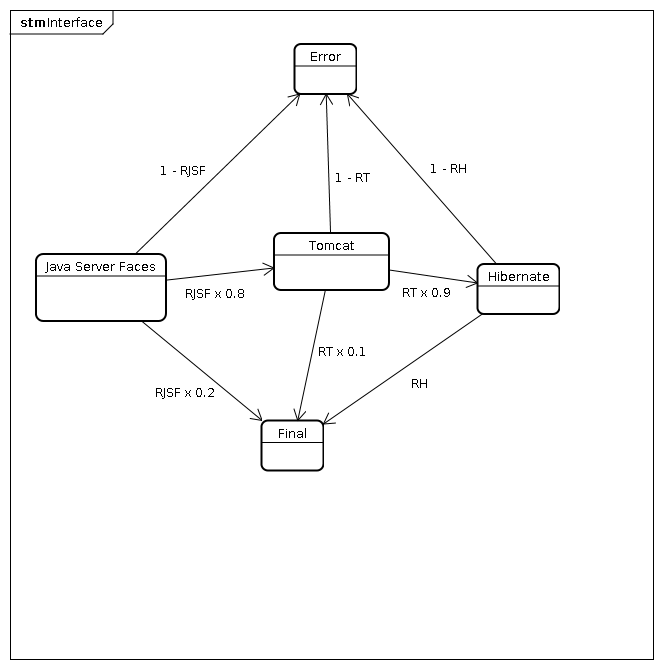
\includegraphics[height=0.7\textheight]{img/Interface}
                \caption{Máquina de estados na Interface}
                \label{fig:sm-interface}
            \end{center}
        \end{figure}

        \framebreak

        \begin{figure}
            \begin{center}
                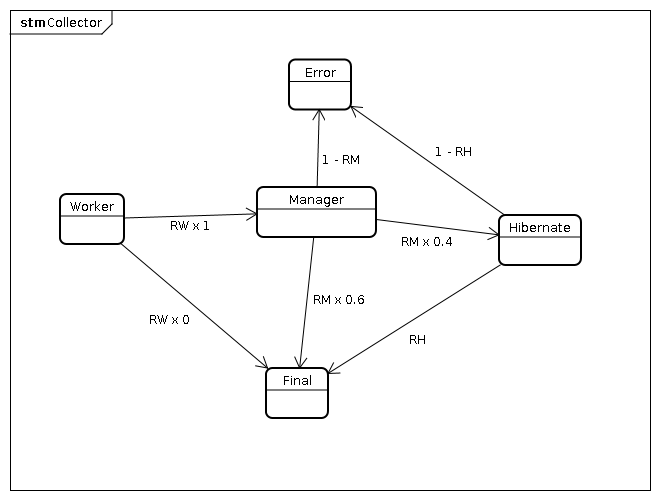
\includegraphics[width=0.7\textwidth]{img/Collector}
                \caption{Máquina de estados no Coletor}
                \label{fig:sm-coletor}
            \end{center}
        \end{figure}

    }

    \subsection{Código Prism}
    \frame{
    
        \frametitle{Código Prism}
        \begin{figure}
            \begin{center}
                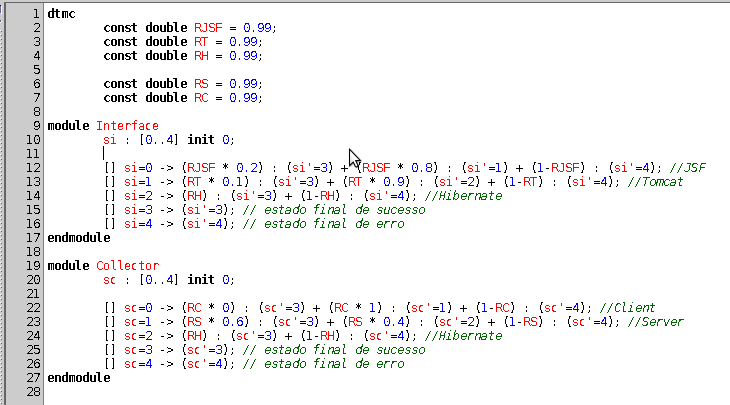
\includegraphics[height=0.7\textheight]{img/prism}
                \caption{Código Prism}
                \label{fig:prism}
            \end{center}
        \end{figure}
    }

    \section{Conclusão}
    

%        \begin{figure}
%            \includegraphics[scale=0.2]{img/figura1.png}
%            \caption{Arquitetura para responder a consultas da Google}
%            \label{fig:arch}
%        \end{figure}


    % =================== Bibliografia ==================== %
    \appendix
    \section*{\appendixname}
    \subsection*{Referências}

    \begin{frame}[allowframebreaks]
      \frametitle{Bibliografia}
        \nocite{*}
        \bibliographystyle{amsplain}
        \bibliography{apresentacao}

    \end{frame}
\end{document}
